\documentclass[border=0pt]{standalone}
\usepackage{pgfplots}
\pgfplotsset{width=\linewidth,compat=1.8}
\usepackage{pgfplotstable}
\usepgfplotslibrary{fillbetween}
\usepackage{amsmath}
\begin{document}

\pgfplotsset{every tick label/.append style={font=\boldmath}}

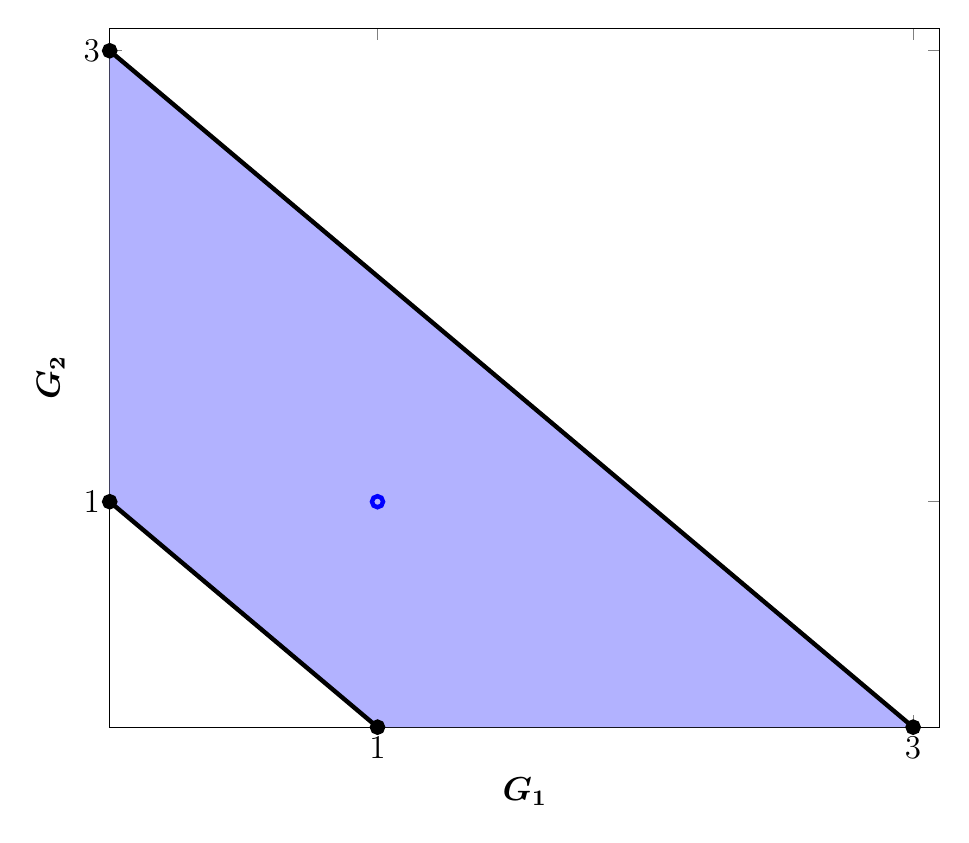
\begin{tikzpicture}
\tikzstyle{every node}=[font=\large]
\begin{axis}[ymax=3.1, ymin=0, xmin=0, xmax=3.1, xlabel= $\boldsymbol{G_1}$, ylabel=$\boldsymbol{G_2}$, xtick={1, 3}, ytick={1, 3},]
    \addlegendimage{red, ultra thick}
    \addlegendimage{blue, ultra thick, dashed}
    \addplot[color=black, ultra thick, mark=*, only marks] coordinates {(0, 3)};
    \addplot[color=black, ultra thick, mark=*, only marks] coordinates {(3, 0)};
    \addplot[color=black, ultra thick, mark=*, only marks] coordinates {(0, 1)};
    \addplot[color=black, ultra thick, mark=*, only marks] coordinates {(1, 0)};
    \addplot[color=blue, ultra thick, mark=o, only marks] coordinates {(1, 1)};
    \addplot[name path=A, color=black, domain=0:1, ultra thick]{1-x};
    \addplot[name path=B, color=black, domain=0:3, ultra thick]{3-x};
    \addplot[blue!30] fill between[of=A and B];
\end{axis}
\end{tikzpicture}
\end{document}